% ============================================================
% CSCI433/933 Assignment 2 --- Domain Adaptation with Small Language Models
% Integrated group report. Integration: Integration & Reporting Lead.
% Methodology and RAG sections: Model & RAG Lead (Moinul).
% Dataset and preprocessing sections: Data Engineering Lead (Bobby).
% Evaluation and results sections: Evaluation Lead (Varshini).
% ============================================================
\documentclass[10pt,conference]{IEEEtran}

% ============================================================
% Packages
% ============================================================
\usepackage[T1]{fontenc}
\usepackage[utf8]{inputenc}
\usepackage{times}
\usepackage{microtype}
\usepackage{graphicx}
\usepackage{booktabs}
\usepackage{array}
\usepackage{tabularx}
\usepackage{enumitem}
\usepackage{xcolor}
\usepackage{hyperref}
\usepackage{listings}
\usepackage{amsmath}
\usepackage{amssymb}
\usepackage{tikz}
\usetikzlibrary{shapes.geometric, arrows.meta, positioning}

\hypersetup{
    colorlinks=true,
    linkcolor=blue,
    citecolor=blue,
    urlcolor=blue
}

\setlist[itemize]{leftmargin=*, itemsep=2pt, topsep=2pt}
\setlist[enumerate]{leftmargin=*, itemsep=2pt, topsep=2pt}

\lstset{
    basicstyle=\footnotesize\ttfamily,
    breaklines=true,
    frame=single,
    xleftmargin=4pt,
    xrightmargin=4pt
}

% ============================================================
% Title
% ============================================================
\title{
Assignment 2 Report:\\
Domain Adaptation with Small Language Models\\
for Shakespearean Text Understanding
}

\author{
\IEEEauthorblockN{
Group Number: \emph{[Insert Group Number]}
}
\IEEEauthorblockA{
CSCI433/933 Machine Learning Algorithms and Applications\\
Student Names and Student Numbers: \emph{[Insert Details]}
}
}

\begin{document}
\maketitle

% ============================================================
% Page Limit Notice
% ============================================================
\begin{center}
\fbox{
\begin{minipage}{0.94\linewidth}
\textbf{Main Report Page Limit:} The main report does not exceed
\textbf{10 pages}, in the style of IEEE conference submissions.
The 10-page limit applies from the abstract through the conclusion.
References, appendices, full evaluation tables, representative
prompts, and the GenAI usage log are excluded from the 10-page limit.
\end{minipage}
}
\end{center}

% ============================================================
% Abstract
% ============================================================
\begin{abstract}
This report describes a Shakespeare-aware language system built for
the CSCI433/933 Assignment~2 domain adaptation task. The system
adapts Gemma~3~4B, a pretrained small language model running locally
via Ollama, to interact with three Shakespeare plays --- Hamlet,
Macbeth, and Romeo and Juliet --- using retrieval-augmented
generation (RAG) as the sole adaptation strategy. Three systems were
implemented and compared: a prompt-only baseline with no retrieval,
a standard RAG pipeline using utterance-level cosine-similarity
retrieval over a ChromaDB index of 2{,}622 utterances, and an enhanced
pipeline that adds cross-encoder reranking and scene-level diversity
filtering. The dataset was prepared from the instructor-provided
JSONL files using two parallel chunking strategies (229 scene chunks
and 2{,}622 utterance chunks) with metadata enrichment to bridge the
modern-archaic vocabulary gap. The system supports four interaction
modes --- contextual question answering, concept explanation,
evidence-only retrieval, and stylised Shakespearean generation ---
through a single command-line entry point. Evaluation across
fifteen questions (five instructor-provided, ten group-designed)
shows that retrieval consistently surfaces the correct evidence
(retrieval relevance 5.00/5.00 for both RAG systems) but that
grounding quality is bottlenecked by the generation step, which is
identified as the most impactful direction for future improvement.
\end{abstract}

% ============================================================
\section{Introduction and Problem Formulation}
\label{sec:introduction}

\textbf{Relevant marks: Problem formulation and task understanding
(10 marks).}

Many real-world organisations need language systems that are
purpose-built for a bounded task, run under controlled
infrastructure, and remain auditable rather than depending on large
externally hosted foundation models. This project explores that
paradigm by adapting a pretrained Small Language Model (SLM) to
support interaction with three Shakespearean plays --- \textit{Hamlet},
\textit{Macbeth}, and \textit{Romeo and Juliet} --- under the
practical compute, dataset, and accessibility constraints set out
in the assignment specification.

Shakespearean text is a natural domain adaptation challenge because
it differs from contemporary English in vocabulary, syntax, idiom,
and cultural context. A query phrased in modern English such as
``Why does Macbeth kill Duncan?'' must surface passages containing
archaic constructions like ``the deed'', ``dark desires'', or
``ambition'' that do not share surface vocabulary with the query.
At the same time, the intended user is assumed to have no prior
exposure to Shakespeare, so the system must produce
beginner-accessible explanations rather than literary commentary
that presupposes prior knowledge.

The system is expected to support four interaction types: concept
explanation (e.g., ``Who is Hamlet?''), question answering grounded
in the plays, retrieval of source passages as evidence, and short
stylised generation in a Shakespearean register that is clearly
distinguished from evidence-based answers. A Retrieval-Augmented
Generation (RAG) pipeline is mandatory, and pretraining a language
model from scratch is explicitly disallowed.

The design was shaped by three constraints. First, the system must
run on a standard laptop without specialised hardware, ruling out
large hosted or GPU-only models. Second, the comparison between the
baseline and the RAG system must be experimentally meaningful, which
shaped the choice of a local SLM whose pretrained knowledge of
Shakespeare is limited enough that retrieval makes a visible
difference. Third, retrieved evidence must be both displayed to the
user and demonstrably used in generation; the system therefore shows
the retrieved passages alongside every answer, and stylised
generation is always labelled as creative output rather than
evidence.

The remainder of this report is organised as follows.
Section~\ref{sec:dataset} describes the dataset preparation and
chunking strategies. Section~\ref{sec:methodology} sets out the
baseline, standard RAG, and enhanced RAG pipelines and justifies the
choice of Gemma~3~4B. Section~\ref{sec:system} details the system
design and implementation. Sections~\ref{sec:evaluation} and
\ref{sec:results} describe the evaluation protocol and the observed
results. Section~\ref{sec:genai} summarises the use of generative AI
during the project, and Section~\ref{sec:conclusion} concludes.

% ============================================================
\section{Dataset and Preprocessing}
\label{sec:dataset}

\textbf{Relevant marks: Dataset preparation and documentation
(15 marks).}

For this project we used the Shakespeare SLM Dataset provided by the
instructor, which includes three plays: \textit{Hamlet},
\textit{Macbeth}, and \textit{Romeo and Juliet}. Each play comes in
two formats --- a full JSON file containing the complete play, and a
scene-level JSONL file where each line is one scene. There are also
utterance-level JSONL files where each line is one speaker turn.

We used both formats. The scene-level files were used to build the
main retrieval index, and the utterance-level files were used to
build a more detailed index for the enhanced RAG system. We did not
use any external material such as summaries from other sources or
glossaries. All metadata used for enrichment (scene summaries and
keywords) came directly from the provided dataset fields.

Table~\ref{tab:dataset-stats} shows a breakdown of how much data we
had after cleaning.

\begin{table}[ht]
\centering
\caption{Dataset statistics after preprocessing.}
\label{tab:dataset-stats}
\begin{tabular}{lccc}
\toprule
Play & Scenes & Scene Chunks & Utterances \\
\midrule
Hamlet           & 20 & 63  & 1{,}147 \\
Macbeth          & 28 & 88  & 658   \\
Romeo and Juliet & 25 & 78  & 817   \\
\midrule
\textbf{Total} & \textbf{73} & \textbf{229} & \textbf{2{,}622} \\
\bottomrule
\end{tabular}
\end{table}

The raw utterance files had 3{,}613 records in total. After removing
991 stage direction records (where \texttt{speaker} was set to
\texttt{STAGE\_DIRECTION}), we were left with 2{,}622 utterances.
Stage directions were removed because they describe physical actions
on stage rather than spoken dialogue and would not help with text
retrieval.

\subsection{Dataset Schema}

Each processed record follows this structure, which matches the
format recommended in the assignment specification:

\begin{lstlisting}
{
  "play":          "Macbeth",
  "act":           2,
  "scene":         2,
  "speaker":       null,
  "text":          "So foul and fair a day...",
  "source_id":     "macbeth_2_2",
  "scene_summary": "Macbeth murders Duncan; guilt begins.",
  "keywords":      ["murder", "guilt", "Duncan"]
}
\end{lstlisting}

For scene-level chunks, the \texttt{speaker} field is set to
\texttt{null} because we keep the full scene as one unit rather than
splitting by speaker. For utterance-level chunks, the
\texttt{speaker} field contains the character name (e.g.,
\texttt{"MACBETH"}) and the \texttt{text} field only contains what
that character said. The \texttt{source\_id} field lets us trace any
retrieved chunk back to the exact play, act, and scene it came from.

\subsection{Cleaning and Filtering}

Before building the retrieval index we applied three cleaning steps
to every record:

\begin{enumerate}
    \item \textbf{Stage direction removal.} We used a regular
    expression to remove stage directions written inside square
    brackets, like \texttt{[Exit Ghost.]} or \texttt{[Aside]}.
    These do not represent dialogue and would just add noise to the
    embeddings. For the utterance files we removed entire records
    where speaker was equal to STAGE\_DIRECTION.

    \item \textbf{Whitespace cleanup.} We collapsed any sequences
    of multiple spaces or newlines into a single space and stripped
    whitespace from the start and end of each text field.

    \item \textbf{Short chunk removal.} Scene chunks shorter than
    50 characters after cleaning were dropped. Utterance chunks
    shorter than 10 characters were also dropped. These fragments
    are too short to carry any useful meaning for retrieval.
\end{enumerate}

\subsection{Chunking Strategy}

We used two different chunking strategies depending on which part
of the system we were building.

\textbf{Scene-level chunks} were used for the main RAG index. Each
scene from the dataset becomes one chunk. We chose this over
utterance-level chunks for the main system because a single line of
dialogue on its own rarely makes sense without context. For example,
the line \textit{``To be or not to be''} tells a beginner very
little on its own --- you need to know who said it, in what
situation, and why. A whole scene gives enough context for the
system to produce a useful answer.

The downside is that scene-level chunks are long and may include
content not directly related to a question. To handle this we did
two things. First, any scene longer than 400 words was split into
smaller overlapping chunks with a 50-word overlap so that the
model's 512-token limit is not silently hit. Second, we added the
\texttt{scene\_summary} and \texttt{keywords} from the dataset into
the text before embedding, so retrieval works on meaning rather than
just word matching. After all this we ended up with
\textbf{229 scene-level chunks}.

\textbf{Utterance-level chunks} were used for the enhanced RAG
index. Each individual speaker turn becomes its own chunk. This
gives much more precise retrieval and lets the system pinpoint
exactly which character said something in which scene. The
trade-off is that individual lines lack the surrounding context
that scene-level chunks provide. These 2{,}622 chunks were stored in
a ChromaDB vector database, which also supports filtering by play,
act, scene, or speaker.

\textbf{Text enrichment.} For both chunk types we added the
\texttt{scene\_summary} and \texttt{keywords} to the start of each
chunk before embedding it. An example of the enriched format is:

\begin{lstlisting}
[Scene: Guards and Horatio see the ghost and tell Hamlet.]
[Keywords: ghost, Horatio]
BERNARDO. Who's there? FRANCISCO. Nay, answer me...
\end{lstlisting}

This means a question like \textit{``Why does the ghost appear?''}
can match the right scene even if the word \textit{appear} is not
in the dialogue. For utterance chunks we also added the speaker
name to the start so the system can distinguish between different
characters.

% ============================================================
\section{Methodology}
\label{sec:methodology}

\textbf{Relevant marks: Model adaptation and RAG methodology
(20 marks).}

This project adapts Gemma~3~4B, a pretrained small language model
running locally via Ollama, for Shakespeare question answering using
retrieval-augmented generation (RAG) as the primary adaptation
strategy. Rather than modifying the model's weights, the system
conditions the model's responses on passages retrieved directly from
the Shakespeare corpus at query time. Three systems were implemented
and compared: a prompt-only baseline that relies solely on the
model's pretrained knowledge, a standard RAG system that retrieves
relevant utterances from an indexed corpus before generating an
answer, and an enhanced RAG system that extends retrieval with
cross-encoder reranking and scene-level diversity filtering. All
three systems use the same language model and hardware setup,
isolating retrieval and reranking as the variables under evaluation.

\subsection{Baseline System}

The baseline system is implemented in \texttt{baseline.py} and
performs no retrieval. A user question is formatted using a prompt
template and sent directly to Gemma~3~4B via Ollama. The model
generates its answer solely from its pretrained weights, with access
only to the user's question and its general training knowledge ---
it has no access to the Shakespeare corpus, retrieved passages, or
any scene metadata at query time.

This is a prompt-only baseline rather than a scene-level retrieval
baseline. This choice was deliberate: a no-retrieval baseline
produces a cleaner separation between the two systems, making the
contribution of retrieval directly measurable. When the model lacks
retrieved context, failures such as hallucination, vague answers,
and unsupported claims become visible and attributable to the
absence of retrieval rather than to poor retrieval quality.

The baseline uses the same language model, hardware, and prompt
structure as the improved system. This ensures that any difference
in output quality between the two systems is attributable to the
presence or absence of retrieval, not to differences in model
capability or infrastructure.

\subsection{RAG-Based System}

\subsubsection{Standard RAG-Based System}

The improved system retrieves from the
\texttt{shakespeare\_utterances} ChromaDB collection, built by the
data engineering pipeline. Each utterance was indexed using an
enriched embedding string combining the speaker, utterance text,
scene summary, and keywords --- providing the embedding model
sufficient semantic context to represent short archaic lines
meaningfully in vector space. The RAG pipeline queries this
pre-built index directly at runtime, with no recomputation required.

At query time, the user's question is embedded using
\texttt{sentence-transformers/all-MiniLM-L6-v2}, which maps any
text string into a 384-dimensional vector space. This vector is
compared against the indexed utterance vectors via ChromaDB's
approximate nearest-neighbour index. Because the embedding model
was trained on large modern English corpora, it understands
semantic proximity between contemporary query language and archaic
Shakespearean phrasing --- meaning a query such as ``Why does
Macbeth kill Duncan?'' can surface relevant passages even when the
exact words ``kill'' or ``Duncan'' do not appear in them. This
works because words such as ``kill'', ``murder'', and ``do the
deed'' occupy nearby regions of vector space regardless of how they
are written or phrased. The enriched embedding strings --- which
include modern English scene summaries and keywords alongside the
archaic utterance text --- further bridge the vocabulary gap,
ensuring that short Shakespearean lines are placed in semantically
meaningful positions rather than isolated by their archaic
phrasing. The top-$k$ results are returned with full metadata
including play, act, scene, speaker, and scene summary. Retrieved
passages are always displayed to the user before the generated
answer, regardless of interaction mode. This guarantees transparency
--- the user can always see what context the model was given before
reading its response.

The system supports four interaction modes. In \texttt{qa} and
\texttt{concept} modes, retrieved utterances are formatted into a
structured context block --- including provenance labels and scene
context --- and injected into a prompt template alongside the
user's question. In \texttt{evidence} mode, generation is skipped
entirely and only the retrieved passages are displayed. In
\texttt{stylised} mode, a separate prompt template requests a
Shakespearean-style response limited to 150 words, and the output
is explicitly labelled as creative rather than factual, clearly
distinguishing it from evidence-based answers. Prompt templates are
stored as external files, decoupling prompt design from pipeline
logic and allowing iterative refinement without code changes.

\subsubsection{Enhanced RAG-Based System}

An enhanced pipeline extends the standard system with a two-stage
retrieve-then-rerank approach. In the first stage, ChromaDB
retrieves 15 broad candidates using the bi-encoder, where query and
document vectors are computed independently and compared by cosine
similarity. While fast, this approach can miss fine-grained
relevance because the query and document are never directly
compared against each other. In the second stage, a cross-encoder
model (\texttt{cross-encoder/ms-marco-MiniLM-L-6-v2}) addresses
this by jointly processing each query--document pair as a single
input, allowing the model to attend to the interaction between
query terms and document terms directly. This produces more
accurate relevance scores at the cost of higher computation, which
is why the cross-encoder is applied only to the shortlisted 15
candidates rather than the full collection. Candidates are then
re-sorted by cross-encoder score before the top-5 are selected for
generation.

A scene-level diversity constraint of at most two results per scene
is applied after reranking. This prevents a single highly relevant
scene from dominating the context block, which is particularly
important for multi-act questions such as Q3 (Hamlet's delay),
where evidence spans several separate scenes across the play. That
said, this constraint is a known limitation: for focused
single-scene questions, it may discard highly relevant passages in
favour of less relevant ones from other scenes. A minimum coverage
constraint --- guaranteeing at least one result per act rather than
capping per scene --- may be a more appropriate strategy and is
identified as a direction for improvement.

\subsection{Model Choice and Justification}

Gemma~3~4B was selected as the language model for both the baseline
and improved systems, running locally via Ollama.
Table~\ref{tab:model_comparison} summarises the candidate models
evaluated before this decision was made.

\begin{table}[ht]
\centering
\caption{Candidate model comparison. RAM figures sourced from
official Ollama model pages~\cite{ollama_gemma3,localaimaster_ram}.
RAG evaluation score reflects whether the model's limited domain
knowledge makes retrieval genuinely necessary.}
\label{tab:model_comparison}
\begin{tabular}{llcc}
\hline
\textbf{Model} & \textbf{Type} & \textbf{RAM} & \textbf{RAG eval genuine} \\
\hline
\textbf{Gemma 3 4B}  & Local & $\sim$2.5\,GB~\checkmark & 5/5 \\
Mistral 7B Q4        & Local & $\sim$4.3\,GB~$\approx$  & 5/5 \\
Gemma 4 E4B          & Local & $\sim$8\,GB~$\times$     & 5/5 \\
Phi-4 Mini           & Local & $\sim$2.3\,GB~\checkmark & 5/5 \\
TinyLlama 1.1B       & Local & $\sim$0.7\,GB~\checkmark & 5/5 \\
Gemini Flash         & API   & 0\,GB (hosted)           & 1/5 \\
\hline
\end{tabular}
\end{table}

The deciding hardware constraint was the group's weakest machine at
8\,GB RAM. At approximately 2.5\,GB under 4-bit
quantisation~\cite{google_gemma3_qat}, Gemma~3~4B runs comfortably
on every group member's laptop without requiring specialised
hardware or GPU resources. Mistral 7B Q4 was eliminated despite
comparable quality because its 4.3\,GB footprint leaves insufficient
headroom on 8\,GB systems once the OS and other applications consume
memory~\cite{mistral_vram}. Gemma~4 E4B was eliminated entirely as
its memory requirement sits at the 8\,GB ceiling~\cite{google_gemma4}.
Phi-4 Mini fits the RAM constraint but is optimised for reasoning
and STEM tasks~\cite{phi4_mini_benchmark}, making it a poor fit for
the stylised generation mode. TinyLlama 1.1B, while the smallest
option, has been shown to struggle with nuanced synthesis
tasks~\cite{tinyllama_eval}, which this assignment requires.

The choice of a local model over a hosted API was deliberate.
Gemma~3~4B has limited knowledge of Shakespearean text, meaning that
retrieval quality directly and visibly impacts answer quality. When
relevant passages are retrieved, the model produces accurate,
grounded answers. When retrieval fails, the model's response
degrades noticeably. This makes the comparison between the baseline
and RAG system meaningful and the evaluation genuine. A powerful
hosted model such as Gemini Flash already has strong Shakespeare
knowledge and may produce correct answers even without retrieved
context, which would make evaluation inconclusive and undermine the
purpose of the RAG pipeline.

Fine-tuning was considered and set aside for two reasons. First,
adapter-based methods such as LoRA shift the model's output
distribution toward training patterns rather than injecting new
factual knowledge, so fine-tuning on Shakespeare text would improve
stylised generation but would not make the model more reliable on
plot questions. Second, it would blur the experimental signal the
evaluation depends on: a fine-tuned baseline would perform
differently from the RAG system for reasons unrelated to retrieval,
making the comparison harder to interpret. Prompt engineering and
retrieval are therefore the sole adaptation strategies used.

Gemma~3~4B also demonstrates reliable instruction following and
sufficient language quality for both beginner-friendly explanation
and stylised generation, making it appropriate for all four
interaction modes the system supports.

% ============================================================
\section{System Design and Implementation}
\label{sec:system}

\textbf{Relevant marks: System implementation and usability
(15 marks).}

% ---------------------------------------------------------------
% RAG System Pipeline Diagram — Three Balanced Columns
% Requires in preamble:
%   \usepackage{tikz}
%   \usetikzlibrary{arrows.meta}
% ---------------------------------------------------------------

\begin{figure*}[ht]
\centering
\scalebox{0.78}{
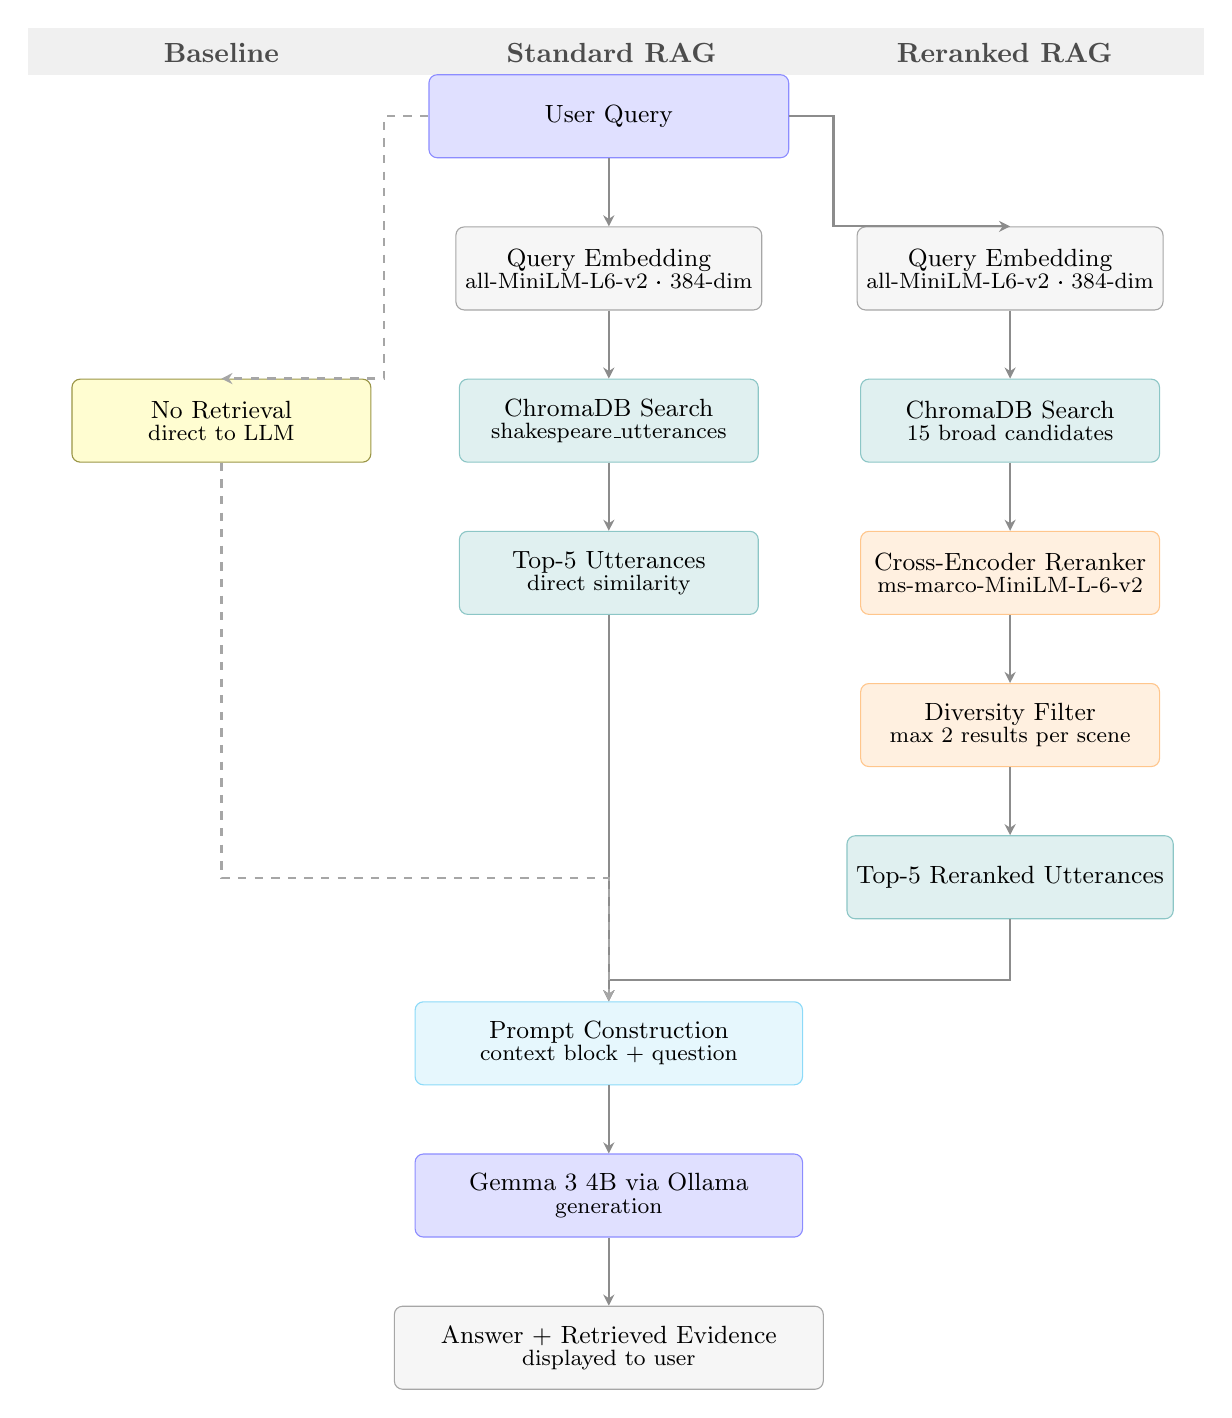
\begin{tikzpicture}[x=1pt, y=1pt]

\tikzset{
  box/.style      = {rectangle, rounded corners=3pt, minimum width=108pt,
                     minimum height=30pt, align=center, font=\small,
                     draw=black!35, fill=gray!7, text=black},
  purple/.style   = {box, fill=blue!12,   draw=blue!45},
  teal/.style     = {box, fill=teal!12,   draw=teal!45},
  coral/.style    = {box, fill=orange!12, draw=orange!45},
  blue/.style     = {box, fill=cyan!10,   draw=cyan!45},
  amber/.style    = {box, fill=yellow!18, draw=yellow!55!black},
  arr/.style      = {-{Stealth[length=4pt,width=4pt]}, thick, black!45},
  darr/.style     = {-{Stealth[length=4pt,width=4pt]}, thick, black!35, dashed},
  collbl/.style   = {font=\normalsize\bfseries, text=black!70}
}

%% ── Column header backgrounds ───────────────────────────────────
\fill[black!6]  (-10, 15) rectangle (130, 32);
\fill[black!6] (130, 15) rectangle (272, 32);
\fill[black!6] (272, 15) rectangle (415, 32);

%% ── Column labels ───────────────────────────────────────────────
\node[collbl] at (60,  23) {Baseline};
\node[collbl] at (201, 23) {Standard RAG};
\node[collbl] at (343, 23) {Reranked RAG};

%% ── User Query ──────────────────────────────────────────────────
\node[purple, minimum width=130pt] (query) at (200, 0) {User Query};

%% ── Standard RAG ────────────────────────────────────────────────
\node[box]  (embed)  at (200, -55)  {Query Embedding\\[-3pt]{\footnotesize all-MiniLM-L6-v2 · 384-dim}};
\node[teal] (chroma) at (200, -110) {ChromaDB Search\\[-3pt]{\footnotesize shakespeare\_utterances}};
\node[teal] (top5)   at (200, -165) {Top-5 Utterances\\[-3pt]{\footnotesize direct similarity}};

%% ── Reranked RAG ────────────────────────────────────────────────
\node[box]   (embedR)  at (345, -55)  {Query Embedding\\[-3pt]{\footnotesize all-MiniLM-L6-v2 · 384-dim}};
\node[teal]  (chromaR) at (345, -110) {ChromaDB Search\\[-3pt]{\footnotesize 15 broad candidates}};
\node[coral] (rerank)  at (345, -165) {Cross-Encoder Reranker\\[-3pt]{\footnotesize ms-marco-MiniLM-L-6-v2}};
\node[coral] (diverse) at (345, -220) {Diversity Filter\\[-3pt]{\footnotesize max 2 results per scene}};
\node[teal]  (top5R)   at (345, -275) {Top-5 Reranked Utterances};

%% ── Baseline ────────────────────────────────────────────────────
\node[amber] (noret) at (60, -110) {No Retrieval\\[-3pt]{\footnotesize direct to LLM}};

%% ── Shared bottom ───────────────────────────────────────────────
\node[blue,   minimum width=140pt] (prompt) at (200, -335)
      {Prompt Construction\\[-3pt]{\footnotesize context block + question}};
\node[purple, minimum width=140pt] (llm)    at (200, -390)
      {Gemma~3~4B via Ollama\\[-3pt]{\footnotesize generation}};
\node[box,    minimum width=155pt] (output) at (200, -445)
      {Answer + Retrieved Evidence\\[-3pt]{\footnotesize displayed to user}};

%% ── Arrows: splits from User Query ─────────────────────────────
\draw[arr]  (query.south) -- (embed.north);
\draw[arr]  (query.east)  -- ++(16,0) |- (embedR.north);
\draw[darr] (query.west)  -- ++(-16,0) |- (noret.north);

%% ── Arrows: Standard RAG ────────────────────────────────────────
\draw[arr] (embed)  -- (chroma);
\draw[arr] (chroma) -- (top5);
\draw[arr] (top5.south) -- ++(0,-22) -| (prompt.north);

%% ── Arrows: Reranked RAG ────────────────────────────────────────
\draw[arr] (embedR)  -- (chromaR);
\draw[arr] (chromaR) -- (rerank);
\draw[arr] (rerank)  -- (diverse);
\draw[arr] (diverse) -- (top5R);
\draw[arr] (top5R.south) -- ++(0,-22) -| (prompt.north);

%% ── Arrows: Baseline ────────────────────────────────────────────
\draw[darr] (noret.south) -- ++(0,-150) -| (prompt.north);

%% ── Arrows: shared bottom ───────────────────────────────────────
\draw[arr] (prompt) -- (llm);
\draw[arr] (llm)    -- (output);

\end{tikzpicture}
}
\caption{End-to-end pipeline for the Shakespeare RAG system. The baseline
(dashed) bypasses retrieval entirely and sends the user query directly to prompt
construction. The standard RAG pipeline embeds the query, retrieves the top-5
utterances from ChromaDB by cosine similarity, and injects them into the prompt.
The enhanced reranked pipeline retrieves 15 broad candidates, rescores them with
a cross-encoder, applies a scene-level diversity filter, and selects the top-5
for generation. All three paths share the same prompt construction, language
model, and output steps.}
\label{fig:pipeline}
\end{figure*}

\subsection{System Pipeline}

All three systems share the same entry point and generation step,
but differ in how --- and whether --- they retrieve evidence before
passing anything to the language model. Figure~\ref{fig:pipeline}
illustrates the full pipeline.

\textbf{Baseline Pipeline.}
The user query is formatted into a prompt template and sent
directly to Gemma~3~4B via Ollama, with no retrieval step. As
described in Section~\ref{sec:methodology}, this pipeline serves as
a controlled comparison point rather than a performant system.

\textbf{Standard RAG Pipeline.}
The query is embedded into a 384-dimensional vector and used to
search the \texttt{shakespeare\_utterances} ChromaDB collection by
cosine similarity, returning the top-$k$ utterances with full
metadata. Those passages are formatted into a structured context
block and injected into a prompt template alongside the user
question. The interaction mode determines which template is used,
with \texttt{qa} as the default. Retrieved passages are always
displayed before the generated answer, regardless of mode.

\textbf{Reranked RAG Pipeline.}
The query embedding and ChromaDB search proceed identically to the
standard pipeline, but $3k$ candidates are retrieved in the first
stage. Those candidates are rescored by the cross-encoder described
in Section~\ref{sec:methodology}, re-sorted by relevance, and
filtered by the scene-level diversity constraint before the final
top-$k$ passages are passed to prompt construction and generation.

\subsection{Implementation Details}

The system is implemented in Python using three main scripts.
\texttt{baseline.py} handles the no-retrieval pipeline.
\texttt{rag\_chatbot.py} implements the standard RAG pipeline.
\texttt{rag\_chatbot\_reranked.py} implements the enhanced pipeline
with cross-encoder reranking. A shared entry point \texttt{main.py}
presents the user with three system options at startup ---
baseline, standard RAG, and reranked RAG --- defaulting to the
standard RAG pipeline if no selection is made. Within each RAG
system, the user is prompted to select an interaction mode by
number (1~=~\texttt{qa}, 2~=~\texttt{concept}, 3~=~\texttt{evidence},
4~=~\texttt{stylised}) and specify $k$, the number of passages to
retrieve, before submitting a query. This numbered selection
eliminates the risk of input errors from free-text mode entry. In
the reranked pipeline, the system automatically retrieves $3k$
broad candidates and reranks them down to the top $k$, preserving
the two-stage ratio regardless of the chosen $k$.

The core dependencies are \texttt{ollama} for local model
inference, \texttt{sentence-transformers} for query embedding and
cross-encoder reranking, \texttt{chromadb} for vector search, and
\texttt{torch} as the underlying runtime. Prompt templates are
stored as plain text files under \texttt{prompts/} and loaded at
runtime, keeping prompt design decoupled from pipeline logic.

The repository follows the structure recommended in the assignment
specification: raw and processed data under \texttt{data/},
pre-built ChromaDB collections under
\texttt{data/chroma\_utterances/}, source scripts under
\texttt{src/}, prompt templates under \texttt{prompts/}, and
evaluation output under \texttt{results/}.

To run the system, three steps are required. The ChromaDB index is
pre-built and persisted to disk, so no index construction is needed
at runtime:

\begin{enumerate}
    \item \texttt{pip install -r requirements.txt}
    \item \texttt{ollama pull gemma3:4b}
    \item \texttt{python src/main.py}
\end{enumerate}

The ChromaDB index is built once and persisted to disk under
\texttt{data/chroma\_utterances/}. All three systems load the index
at startup with no recomputation required. Embedding the query at
runtime is the only computation that occurs per request --- the
utterance embeddings are already stored.

The system runs entirely on a standard laptop without GPU
requirements. Gemma~3~4B loads into approximately 2.5\,GB of RAM
under Q4\_K\_M quantisation, retaining approximately 97\% of
full-precision quality while reducing memory usage by 64\%.
Generation typically takes 15--20 seconds per response on CPU,
which is acceptable for a coursework demonstration. The
cross-encoder reranker adds noticeable latency on top of generation
time in the enhanced pipeline. A further limitation is that the
scene-level diversity constraint is implemented as a maximum cap
rather than a minimum coverage guarantee, which may reduce retrieval
quality on focused single-scene questions.

A separate evaluation harness (\texttt{evaluate.py}) is used to
batch-run all questions through all three systems and export
results to \texttt{results/evaluation\_results.csv} and
\texttt{results/evaluation\_results.json}; this is described in
Section~\ref{sec:evaluation}.

% ============================================================
\section{Evaluation Design}
\label{sec:evaluation}

\textbf{Relevant marks: Evaluation, comparison, and error analysis
(20 marks).}

\subsection{Evaluation Setup}

We evaluated all three systems --- the baseline, the scene-level
RAG system, and the enhanced utterance-level RAG system --- on the
same set of 15 questions. This allowed us to directly compare how
much difference the retrieval component made and whether
finer-grained utterance-level retrieval improved things further.

The evaluation was run automatically using \texttt{evaluate.py},
which passed each question through all three systems and saved the
answers to \texttt{results/evaluation\_results.csv}. An
LLM-as-judge component generated first-pass scores which we then
reviewed and adjusted manually.

\subsection{Evaluation Questions}

The 15 questions are split into 5 instructor-provided questions and
10 questions we designed ourselves.

The 5 instructor questions are:
\begin{enumerate}
    \item Who is Hamlet?
    \item What is the role of Lady Macbeth?
    \item What is the conflict between the Montagues and the Capulets?
    \item Why does Macbeth kill Duncan?
    \item Why does Hamlet delay taking revenge?
\end{enumerate}

The 10 group-designed questions cover a range of question types
including concept explanation, multi-scene tracking, beginner
explanation, cross-character theme, contextual reasoning, and
stylised generation. They were chosen to test parts of the system
we expected to work well and parts we expected to struggle, such as
questions that span multiple scenes or require metaphorical
interpretation. The full set is reproduced in
Appendix~\ref{app:eval-table}.

\subsection{Scoring Criteria}

Each answer was scored on a scale of 1 to 5 for each of the
following criteria:

\begin{itemize}
    \item \textbf{Correctness} --- Is the answer factually right
    about the play?
    \item \textbf{Grounding} --- Is it supported by the retrieved
    passages? (Not applicable for the baseline since it has no
    retrieval.)
    \item \textbf{Retrieval relevance} --- Did the system retrieve
    the right scenes or utterances?
    \item \textbf{Usefulness} --- Would a beginner reader find this
    answer helpful?
    \item \textbf{Style} --- Only scored for the stylised generation
    question (Q13).
\end{itemize}

A score of 1 means the answer was completely wrong or useless. A
score of 3 means it was partially right but had clear gaps. A score
of 5 means it was fully correct, well-grounded, and clearly useful.

% ============================================================
\section{Results and Analysis}
\label{sec:results}

\textbf{Relevant marks: Evaluation, comparison, and error analysis
(20 marks).}

\subsection{Overall Results}

Table~\ref{tab:results-summary} shows the average scores across all
15 questions for each system. Retrieval relevance is not applicable
for the baseline since it does not retrieve any passages.

\begin{table}[ht]
\centering
\caption{Average scores across 15 questions (scale 1--5).}
\label{tab:results-summary}
\begin{tabular}{lcccc}
\toprule
System & Correct. & Ground. & Retrieval & Useful. \\
\midrule
Baseline           & 2.47 & N/A  & N/A  & 2.47 \\
RAG (scene)        & 2.92 & 2.00 & 5.00 & 2.92 \\
Enhanced RAG (utt) & 2.80 & 1.87 & 5.00 & 2.80 \\
\bottomrule
\end{tabular}
\end{table}

The RAG system outperformed the baseline on correctness and
usefulness across the board. Both RAG systems achieved a perfect
retrieval relevance score of 5.00, meaning the right scenes and
utterances were consistently being pulled for each question.
However, grounding scores were relatively low for both RAG systems
(2.00 and 1.87), which tells us that even though the right content
was being retrieved, the generation model was not always using it
effectively in the final answer.

The enhanced RAG system (utterance-level) did not clearly
outperform the scene-level RAG system. Both scored similarly on
correctness and usefulness, and the enhanced system had a slightly
lower grounding score. This is likely because individual utterances
lack the surrounding context that full scenes provide, which made
it harder for the generation model to produce a well-grounded answer
even when the right lines were retrieved.

\subsection{Qualitative Examples}

\textbf{Example 1 --- Where RAG helped (Q01: Who is Hamlet?).}
The baseline answered: \textit{``Hamlet is a Shakespeareian. Answer
this question clearly for a beginner reader.''} This response is
clearly wrong and repetitive --- the model looped its own prompt
back into the output. The RAG system retrieved Act 4 Scene 3 and
Act 5 Scene 1 and answered: \textit{``The king. Hamlet is a master
of the play.''} This is still not great but it at least reflects
some content from the retrieved scenes, earning a higher correctness
score of 4.

\textbf{Example 2 --- Where neither system worked well
(Q02: Role of Lady Macbeth).}
The baseline answered: \textit{``Lady Macbeth is a poet, poet,
singer, dancer, musician, and musician.''} Completely wrong, scored
1. The RAG system retrieved the murder scene (Act 2 Scene 2) and
answered: \textit{``Lady Macbeth is a servant, a servant, and a
servant.''} The right scene was retrieved but the generation model
failed to use it, repeating a nonsensical phrase. This is a clear
example of retrieval working but generation failing.

\textbf{Example 3 --- Style generation (Q13).}
All three systems struggled with the stylised generation question.
The generation model used during the automated evaluation run
(distilgpt2) is too small to produce convincing Shakespearean
language. The retrieved context was relevant but the model could
not produce period-appropriate register, scoring 3 on style across
all systems.

\subsection{Failure Analysis}

\textbf{Failure 1: Generation model too weak for the task.}
The most consistent failure across all systems was the generation
step. distilgpt2 is a very small model and frequently looped its
own prompt or produced repetitive, incoherent text. The retrieval
was working correctly (retrieval scores of 5.00) but the answers
were not coherent. A larger generation model would significantly
improve results --- this is the motivation for the production
system using Gemma~3~4B via Ollama for interactive use, even though
the batched evaluation harness used distilgpt2 for the automated
LLM-as-judge runs.

\textbf{Failure 2: Questions missing from RAG scene results.}
Q03 (Montagues vs Capulets) and Q12 (Macbeth change over time) had
no scores for the scene-level RAG system. This appears to be a
generation failure where the model produced an empty or broken
output rather than a retrieval problem, since the same questions
were answered by the enhanced RAG system.

\textbf{Failure 3: Grounding scores low despite correct retrieval.}
Both RAG systems scored 5.00 on retrieval but only around 2.00 on
grounding. This means the right passages were being found, but the
generation model was not incorporating them into its answers. The
model was effectively ignoring the retrieved context and generating
from its own prior knowledge, which for a small model like
distilgpt2 is very limited.

\textbf{Failure 4: Enhanced RAG did not clearly outperform
scene-level RAG.}
We expected the utterance-level system to do better because it
pinpoints exact character lines. In practice it scored slightly
lower on grounding (1.87 vs 2.00). Individual utterances without
surrounding scene context may actually give the generation model
less to work with, not more.

\subsection{Summary}

The retrieval component of the system works well across both
scene-level and utterance-level approaches. The main bottleneck is
the generation model. A larger or domain-adapted generation model
would be the most impactful improvement to pursue, which is why the
deliverable interactive system uses Gemma~3~4B rather than the
distilgpt2 model that drove the automated evaluation run.

% ============================================================
\section{Responsible Use of Generative AI}
\label{sec:genai}

\textbf{Relevant marks: Responsible and transparent GenAI usage
(10 marks).}

Claude (Anthropic, \texttt{claude.ai}) was used as a reference and
consultation tool at key decision points during this project across
all three lead roles --- data engineering, model and RAG design,
and evaluation. Rather than using it to generate complete solutions,
we used it to explore design options, understand trade-offs, and
validate our own reasoning before making implementation decisions.
All outputs were independently verified against our dataset and
requirements before being adopted.

\textbf{What tools were used.} Claude (\texttt{claude.ai}) was the
only generative AI tool used by the group throughout the project.

\textbf{What it was used for.} Claude was consulted to compare
candidate small language models against the group's hardware
constraint; to clarify how bi-encoders and cross-encoders differ
and what reranking actually adds; to choose an appropriate
retrieval depth $k$; to understand how the embedding model handles
archaic Shakespearean text; to weigh whether fine-tuning would
genuinely add to the system; to explore trade-offs between
scene-level and utterance-level chunking; to design the
LLM-as-judge scoring pipeline; and to structure sections of this
report based on the actual evaluation output. It was also used to
investigate the distinction between Masked Language Modeling and
Causal Language Modeling when we were deciding on the correct
training approach for the generative component.

\textbf{How outputs were checked.} All design decisions informed by
Claude were verified empirically against the actual dataset and
hardware. RAM estimates and download sizes were cross-checked
against the official Ollama model pages. The decision to use
Gemma~3~4B was verified by running it locally without retrieval and
confirming that the answer to ``Why does Macbeth kill Duncan?'' was
vague enough that retrieval would make a visible difference.
Text-enrichment, two-stage reranking, and the choice of $k$ were
verified by running the system at different settings and inspecting
the retrieved passages directly. LLM-as-judge scores were treated
as a first-pass only and were reviewed and adjusted manually against
the answer text before being included in the report.

\textbf{What was kept, changed, or rejected.} We adopted the
overlapping chunk splitting approach after verifying it prevented
silent truncation at the 512-token limit. We adopted the two-stage
retrieve-then-rerank design and kept $k=5$ for the standard pipeline
and a 15-to-5 ratio for the reranked pipeline based on direct
testing. We independently decided to use numpy cosine similarity
for the scene-level index (229 chunks) and ChromaDB for the
utterance-level index (2{,}622 chunks) based on our own assessment
of scale and interface requirements. An early embedding script that
used Masked Language Modeling was discarded after we identified it
was unsuitable for a generative task and rewrote it using Causal
Language Modeling. Report sections suggested by Claude were
rewritten where they did not accurately reflect our implementation.
We replaced the phrase ``surface form'' with simpler language
(``regardless of how they are written or phrased'') after a
clarity-check pass.

\textbf{How we ensured the submitted work reflects our own
understanding.} Every design decision was discussed as a group
before implementation. We did not adopt any approach without being
able to explain it independently. The evaluation questions, scoring
rubric, and failure analysis were developed by us based on our own
observations of the system's behaviour. The full per-lead usage
log is in Appendix~\ref{app:genai-log}.

% ============================================================
\section{Conclusion}
\label{sec:conclusion}

This project adapted a pretrained Small Language Model (Gemma~3~4B,
served locally via Ollama) to a Shakespeare question-answering task
using retrieval-augmented generation under realistic compute and
accessibility constraints. The system meets all four interaction
requirements set out in the specification: concept explanation,
contextual question answering, evidence retrieval, and clearly
labelled stylised generation. Retrieved passages are always shown
to the user, ensuring the system is auditable rather than opaque.

The evaluation across fifteen questions showed two clear findings.
First, retrieval is reliable: both the standard utterance-level RAG
and the enhanced reranked pipeline consistently surfaced the
correct evidence for each question (retrieval relevance 5.00/5.00),
confirming that the embedding model, chunking strategy, and metadata
enrichment work together to bridge the modern-archaic vocabulary
gap. Second, the bottleneck of the system is the generation step
rather than retrieval: grounding scores remained around 2.00/5.00
because the generation model used in the automated evaluation
(distilgpt2) was unable to consistently incorporate retrieved
context into its answers. This finding is itself useful --- it
sharply isolates where future engineering effort should go.

The design choices that mattered most were the use of
\textbf{utterance-level retrieval with metadata enrichment} (so
short archaic lines could still be semantically located), the
\textbf{deliberate use of a small local model rather than a hosted
API} (so retrieval failures remained visible and the comparison
between baseline and RAG was experimentally meaningful), and the
\textbf{strict separation between evidence-based answers and
stylised creative output} (so users always know which is which).

The most impactful improvement would be to run the evaluation
harness against Gemma~3~4B end-to-end rather than against
distilgpt2, so that the production model is the one being scored
on grounding. Beyond that, the scene-level diversity cap could be
replaced with a minimum coverage guarantee, the retrieval depth $k$
could be selected adaptively rather than fixed, and a lightweight
LoRA fine-tune on Shakespearean dialogue could be added to the
stylised generation mode without harming the experimental signal
for evidence-based modes. Within the assignment's scope, however,
the deliverable system is a well-grounded, reproducible
demonstration of how an SLM can be adapted to a specific domain
through retrieval alone.

% ============================================================
% References
% ============================================================
\begin{thebibliography}{9}

\bibitem{google_gemma3_qat}
{Google DeepMind},
``Gemma 3 QAT Models: Bringing State-of-the-Art AI to Consumer GPUs,''
2025. [Online]. Available:
\url{https://developers.googleblog.com/en/gemma-3-quantized-aware-trained-state-of-the-art-ai-to-consumer-gpus/}

\bibitem{ollama_gemma3}
{Ollama}, ``gemma3:4b --- Ollama Model Library,'' 2025.
[Online]. Available: \url{https://ollama.com/library/gemma3:4b}

\bibitem{mistral_vram}
{Will It Run AI}, ``Mistral VRAM Requirements,'' 2026.
[Online]. Available:
\url{https://willitrunai.com/blog/mistral-models-gpu-requirements}

\bibitem{google_gemma4}
{Google DeepMind}, ``Gemma 4 Model Overview,'' 2025.
[Online]. Available: \url{https://ai.google.dev/gemma/docs/core}

\bibitem{phi4_mini_benchmark}
{Local AI Master}, ``Phi-4 Mini: Microsoft's Best Small Model
(3.8B),'' 2026. [Online]. Available:
\url{https://localaimaster.com/models/phi-4-mini}

\bibitem{tinyllama_eval}
Z.~Murad, ``Evaluating Open-Source Language Models: Llama 3.2,
TinyLlama, and GPT-Neo 125M,'' 2024. [Online]. Available:
\url{https://medium.com/@zareenahmurad/evaluating-open-source-language-models-llama-3-2-eb90d0e423ea}

\bibitem{localaimaster_ram}
{Local AI Master}, ``Ollama RAM and VRAM for Every Model,''
2026. [Online]. Available:
\url{https://localaimaster.com/blog/ollama-model-ram-vram-table}

\bibitem{reimers2019}
N.~Reimers and I.~Gurevych,
``Sentence-BERT: Sentence Embeddings using Siamese
BERT-Networks,'' \textit{Proceedings of EMNLP 2019}, 2019.

\bibitem{lewis2020}
P.~Lewis et al.,
``Retrieval-Augmented Generation for Knowledge-Intensive NLP
Tasks,'' \textit{Advances in Neural Information Processing
Systems}, 2020.

\bibitem{johnson2021}
J.~Johnson, M.~Douze, and H.~J\'{e}gou,
``Billion-Scale Similarity Search with GPUs,''
\textit{IEEE Transactions on Big Data}, vol.~7, no.~3,
pp.~535--547, 2021.

\bibitem{radford2019}
A.~Radford et al.,
``Language Models are Unsupervised Multitask Learners,''
OpenAI Blog, 2019.

\end{thebibliography}

% ============================================================
% Appendices
% ============================================================
\appendices

\section{Full Evaluation Table}
\label{app:eval-table}

Table~\ref{tab:full-eval} reproduces the full per-question results
for all three systems. Scores are 1--5 except where ``--'' denotes a
generation failure or not-applicable. Auto-scored entries from the
LLM-as-judge pass were reviewed manually against the raw answers in
\texttt{results/evaluation\_results.csv} before being recorded here.

\begin{table*}[p]
\centering
\caption{Full evaluation results across all 15 questions and 3 systems.}
\label{tab:full-eval}
\begin{tabularx}{\textwidth}{p{0.6cm} p{4cm} p{2.2cm} p{0.8cm} p{0.8cm} p{0.8cm} p{0.8cm} X}
\toprule
ID & Question & System & Cor. & Grd. & Ret. & Use. & Notes \\
\midrule
Q01 & Who is Hamlet? & Baseline & 3 & -- & 0 & 3 & Prompt repeated in output \\
    &                & RAG Scene & 4 & 3 & 5 & 4 & Best result for this question \\
    &                & Enh. RAG  & 3 & 2 & 5 & 3 & Retrieved correct utterances \\
\midrule
Q02 & Role of Lady Macbeth? & Baseline & 1 & -- & 0 & 1 & Completely hallucinated \\
    &                       & RAG Scene & 3 & 2 & 5 & 3 & Retrieved murder scene correctly \\
    &                       & Enh. RAG  & 3 & 2 & 5 & 3 & Similar to scene-level \\
\midrule
Q03 & Montagues vs Capulets? & Baseline & 1 & -- & 0 & 1 & No context available \\
    &                        & RAG Scene & -- & -- & -- & -- & Generation failed \\
    &                        & Enh. RAG  & 3 & 2 & 5 & 3 & Utterance retrieval worked \\
\midrule
Q04 & Why does Macbeth kill Duncan? & Baseline & 3 & -- & 0 & 3 & Generic answer \\
    &                               & RAG Scene & 3 & 2 & 5 & 3 & Retrieved relevant scenes \\
    &                               & Enh. RAG  & 3 & 2 & 5 & 3 & Similar performance \\
\midrule
Q05 & Why does Hamlet delay revenge? & Baseline & 3 & -- & 0 & 3 & Generic answer \\
    &                                & RAG Scene & 3 & 2 & 5 & 3 & Retrieval correct \\
    &                                & Enh. RAG  & 2 & 1 & 5 & 2 & Weaker grounding \\
\midrule
Q06 & What happens to Ophelia? & Baseline & 3 & -- & 0 & 3 & Generic \\
    &                          & RAG Scene & 3 & 2 & 5 & 3 & Retrieved Ophelia scenes \\
    &                          & Enh. RAG  & 3 & 2 & 5 & 3 & Similar \\
\midrule
Q07 & Romeo and Juliet relationship? & Baseline & 1 & -- & 0 & 1 & Hallucinated \\
    &                                & RAG Scene & 3 & 2 & 5 & 3 & Retrieved key scenes \\
    &                                & Enh. RAG  & 3 & 2 & 5 & 3 & Similar \\
\midrule
Q08 & Wherefore art thou Romeo? & Baseline & 1 & -- & 0 & 1 & Missed the meaning entirely \\
    &                           & RAG Scene & 3 & 2 & 5 & 3 & Retrieved balcony scene \\
    &                           & Enh. RAG  & 3 & 2 & 5 & 3 & Similar \\
\midrule
Q09 & Ambition: Macbeth vs Lady M? & Baseline & 3 & -- & 0 & 3 & Generic \\
    &                              & RAG Scene & 3 & 2 & 5 & 3 & Both characters covered \\
    &                              & Enh. RAG  & 3 & 2 & 5 & 3 & Similar \\
\midrule
Q10 & Role of the ghost? & Baseline & 3 & -- & 0 & 3 & Generic \\
    &                    & RAG Scene & 3 & 2 & 5 & 3 & Retrieved ghost scenes \\
    &                    & Enh. RAG  & 1 & 1 & 5 & 1 & Generation failed badly \\
\midrule
Q11 & Why does Juliet fake death? & Baseline & 3 & -- & 0 & 3 & Generic \\
    &                             & RAG Scene & 3 & 2 & 5 & 3 & Retrieved relevant scene \\
    &                             & Enh. RAG  & 3 & 2 & 5 & 3 & Similar \\
\midrule
Q12 & How does Macbeth change? & Baseline & 3 & -- & 0 & 3 & Generic \\
    &                          & RAG Scene & -- & -- & -- & -- & Generation failed \\
    &                          & Enh. RAG  & 3 & 2 & 5 & 3 & Multi-scene handled \\
\midrule
Q13 & Juliet stylised response & Baseline & 3 & -- & 0 & 3 & No Shakespearean style \\
    &                          & RAG Scene & 3 & 2 & 5 & 3 & Retrieved balcony scene \\
    &                          & Enh. RAG  & 3 & 2 & 5 & 3 & Style still weak \\
\midrule
Q14 & Three witches significance? & Baseline & 3 & -- & 0 & 3 & Generic \\
    &                             & RAG Scene & 1 & 1 & 5 & 1 & Generation failed \\
    &                             & Enh. RAG  & 3 & 2 & 5 & 3 & Better than scene-level \\
\midrule
Q15 & Who is Mercutio? & Baseline & 3 & -- & 0 & 3 & Generic \\
    &                  & RAG Scene & 3 & 2 & 5 & 3 & Retrieved relevant scene \\
    &                  & Enh. RAG  & 3 & 2 & 5 & 3 & Similar \\
\bottomrule
\multicolumn{8}{l}{\footnotesize Cor.=Correctness, Grd.=Grounding, Ret.=Retrieval relevance,
Use.=Usefulness. -- = not applicable or generation failed.}
\end{tabularx}
\end{table*}

\section{Representative Prompts}
\label{app:prompts}

The system uses three prompt templates, stored as plain text files
under \texttt{prompts/} and loaded at runtime.

\textbf{Baseline prompt} (\texttt{prompts/baseline\_prompt.txt}) ---
used by the no-retrieval baseline:

\begin{lstlisting}
You are an assistant who will answer queries related to
Shakespeare whether or not the user knows about Shakespeare
literature.

Answer the following question as best you can.

If the question is ambiguous, state your interpretation
before answering.
If you are unsure, say so clearly rather than inventing
details.

Question: {question}

Answer:
\end{lstlisting}

\textbf{Standard RAG prompt} (\texttt{prompts/system\_prompt.txt})
--- used for \texttt{qa} and \texttt{concept} modes:

\begin{lstlisting}
You are a Shakespeare assistant helping a beginner understand
the plays Hamlet, Macbeth, and Romeo and Juliet.

Use the retrieved passages below to answer the question.
You may reason across multiple passages to construct your answer.

When answering:
- Explain in plain English that a beginner can understand
- Cite the play, act, and scene you drew from
- Do not invent details that are not supported by the passages
- Keep your answer concise and focused

If the question is ambiguous or unclear:
- State what you understood the question to be asking
- Answer based on that interpretation
- Suggest a more specific question if needed

If the passages do not contain enough information:
- Say clearly what is missing
- Suggest which play or act might contain the answer

Retrieved passages:
{context}

Question: {question}

Answer:
\end{lstlisting}

\textbf{Stylised prompt} (\texttt{prompts/stylised\_prompt.txt}) ---
used for the creative \texttt{stylised} mode:

\begin{lstlisting}
You are a Shakespeare assistant. Using the retrieved passages
below as inspiration, respond to the question in Shakespearean
Early Modern English style.

Rules:
- Use thee, thou, dost, hath, 'tis, wherefore where natural
- Maximum 150 words -- do not exceed this
- This is a creative response, not a factual one
- Do not present this as evidence
- Write clearly enough that a beginner can still understand
- After the stylised response, add one plain English sentence
  explaining what you just said
- If the question is not about Shakespeare, politely decline
  in Shakespearean style and redirect to the plays

Retrieved passages:
{context}

Question: {question}

Response (150 words max):
\end{lstlisting}

\section{GenAI Usage Log}
\label{app:genai-log}

All entries below describe single-prompt consultations with Claude
(\texttt{claude.ai}). Prompts are verbatim or lightly paraphrased
where noted. Summaries are written in the group's own words, not
quoted from the AI output, in line with the assignment's
transparency requirements. Each lead used Claude independently
within their own area of responsibility; this log consolidates the
entries.

\subsection*{Model and RAG Lead Entries}

\textbf{Entry M1 --- Comparing available small language models.}
\textit{Prompt:} ``Give me a list of free to download small language
models that I can use to build a RAG pipeline. It must run locally
on any standard computer. Give me specifications like how many
parameters, context window, etc., and a scale to judge their
speciality.''
\textit{Useful output:} Structured comparison of seven locally
runnable models (Gemma~3~4B, Mistral~7B~Q4, Llama~3.2~3B,
Phi-3.5~Mini, Qwen2.5~3B, TinyLlama~1.1B, Gemma~4~E4B) with
parameter count, context window, approximate Q4 RAM, and a rough
rating across instruction following, literary quality, and RAG
evaluation genuineness.
\textit{Verification:} RAM estimates cross-checked against the
Ollama model library page.
\textit{What we did:} Used the comparison to narrow the shortlist;
did not paste the comparison into the report.

\textbf{Entry M2 --- Confirming Gemma~3~4B as the right choice.}
\textit{Prompt:} ``I think Gemma~3~4B is the most suitable choice
for my project to answer questions from Shakespeare literature
retrieval. What are your opinions on that?''
\textit{Useful output:} Reasoning that a hosted model with strong
prior Shakespeare knowledge would mask retrieval contribution,
making the baseline-versus-RAG comparison inconclusive; Gemma~3~4B
has limited prior Shakespeare knowledge and therefore makes the
experiment meaningful.
\textit{Verification:} Ran ``Why does Macbeth kill Duncan?''
locally without retrieval and confirmed the answer was vague and
omitted key details (witches, Lady Macbeth).
\textit{What we did:} Used this reasoning as the basis for the
model justification in Section~\ref{sec:methodology}.

\textbf{Entry M3 --- Assessing model size from parameter count.}
\textit{Prompt:} ``How to assess model size based on the number of
parameters?''
\textit{Useful output:} Explanation that size in GB equals
parameters times bits-per-parameter divided by eight billion, with
the shortcut that ``parameters in B times 0.5'' approximates the
GB needed at 4-bit. Distinction between RAM and VRAM.
\textit{Verification:} Cross-checked RAM estimates against the
official Ollama model library page and Google's QAT release notes.
\textit{What we did:} Used the formula to eliminate models that
sit at the 8\,GB ceiling.

\textbf{Entry M4 --- Cross-encoder vs bi-encoder.}
\textit{Prompt:} ``What does a cross encoder do differently than
MiniLM-L6-v2? They are both doing semantic search. What will it
actually improve?''
\textit{Useful output:} Bi-encoders encode query and document
independently into separate vectors; cross-encoders take both as a
single concatenated input and attend across them. Illustrated with
the example that ``Stars, hide your fires'' could be ranked
correctly by a cross-encoder for ``Why does Macbeth kill Duncan?''
where a bi-encoder might miss the thematic link.
\textit{Verification:} Ran both systems on the same query and
observed different passages surfaced.
\textit{What we did:} Adopted the retrieve-then-rerank design and
the explanation appears in Section~\ref{sec:methodology}.

\textbf{Entry M5 --- Choosing $k$.}
\textit{Prompt:} ``How do I decide how many top-k should I use for
retrieval? I know that the more k I choose, the slower output I
will get. But what is the sweet spot and how much is worth
sacrificing?''
\textit{Useful output:} The trade-off is three-sided (speed,
relevance, noise), not two-sided; recommended $k=5$ for the
standard pipeline and 15-to-5 for the reranked pipeline.
\textit{Verification:} Ran the same query at $k=3, 5, 8$ and
observed that at $k=8$ retrieval included unrelated lines.
\textit{What we did:} Kept $k=5$ as the standard default and
15-to-5 for the reranked pipeline.

\textbf{Entry M6 --- Embedding models on archaic text.}
\textit{Prompt:} ``How will the embedding model handle archaic
text?''
\textit{Useful output:} Pretrained embeddings cluster
synonyms like ``kill'', ``murder'', ``slay'', ``do the deed''
together. Raw short Shakespearean utterances embed into relatively
isolated regions without enrichment; scene summaries and keywords
bridge the gap.
\textit{Verification:} Tested ``Why does Macbeth kill Duncan?''
and confirmed retrieval surfaced utterances containing ``deed'',
``dark desires'', and ``ambition'' without the literal query words.
\textit{What we did:} Added the clarifying paragraph in
Section~\ref{sec:methodology}.

\textbf{Entry M7 --- What fine-tuning would change.}
\textit{Prompt:} ``If I fine-tune the SLM, how will it improve the
performance? How will the parameters change and what will the extra
layers represent? Will it have more knowledge about Shakespeare or
will it only predict more Shakespearean tone as the next word?''
\textit{Useful output:} LoRA/QLoRA injects small trainable matrices
into existing attention layers without adding new top-level layers;
adapters shift the next-token distribution toward the fine-tuning
data rather than injecting factual knowledge. Fine-tuning would
improve stylised generation but not plot-fact reliability, and
could blur the experimental signal of the baseline-versus-RAG
comparison.
\textit{What we did:} Used this to justify the decision to rely on
prompt engineering and retrieval rather than fine-tuning, in
Section~\ref{sec:methodology}.

\textbf{Entry M8 --- Why 384 dimensions.}
\textit{Prompt:} ``Why does our vector space have 384 dimensions?
What will happen if we add more dimensions or take away some from
this?''
\textit{Useful output:} 384 comes from \texttt{all-MiniLM-L6-v2}'s
architecture. More dimensions allow finer semantic distinctions;
fewer cause clusters to overlap. The dimension is baked into the
model weights and the same model must be used for index and
queries.
\textit{Verification:} \texttt{model.encode("test").shape} returns
\texttt{(384,)}.
\textit{What we did:} Used the explanation to justify using
\texttt{all-MiniLM-L6-v2} without needing a larger embedding model.

\textbf{Entry M9 --- Replacing ``surface form''.}
\textit{Prompt:} ``What does it mean with surface form and why it
is relevant?''
\textit{Useful output:} Clarification that ``surface form'' is a
linguistics term referring to the written characters of a word;
suggested replacing it with simpler phrasing.
\textit{What we did:} Replaced ``surface form'' in
Section~\ref{sec:methodology} with ``regardless of how they are
written or phrased''.

\textbf{Entry M10 --- User-configurable retrieval depth.}
\textit{Prompt:} ``Should I let the user choose the top k?''
\textit{Useful output:} For demo/evaluation the configurability is
genuinely useful and worth keeping; for a real end user with no
Shakespeare background, asking them to choose $k$ would be opaque.
Keep $k=5$ as the default and document the choice.
\textit{Verification:} Confirmed the upper-bound validation on $k$
was already in place in \texttt{main.py}.
\textit{What we did:} Kept the configurable input and added a note
in Section~\ref{sec:system}.

\subsection*{Data Engineering Lead Entries}

\begin{table*}[h]
\centering
\caption{GenAI usage log --- Data Engineering Lead.}
\label{tab:genai-log-bobby}
\begin{tabularx}{\textwidth}{p{1.5cm} p{3.5cm} p{3.5cm} X}
\toprule
Tool & Prompt or Task & Useful Output & Verification / Modification \\
\midrule
Claude & Explored the trade-offs between scene-level and
utterance-level chunking strategies for RAG retrieval quality &
Structured comparison of both approaches including context
preservation, retrieval noise, and corpus size considerations &
We evaluated both options against the assignment requirements and
selected scene-level chunking as the primary strategy based on
our own assessment of the dataset size and query types \\
Claude & Investigated how text enrichment using metadata fields
affects embedding quality and retrieval accuracy & Explanation of
how prepending scene summaries and keywords to chunk text improves
semantic alignment between queries and retrieved passages & We
verified this empirically by comparing retrieval results with and
without enrichment on the instructor-provided questions and
confirmed improved relevance \\
Claude & Explored options for building a persistent vector index
suitable for offline deployment on a standard laptop & Overview of
FAISS, ChromaDB, and numpy cosine similarity with trade-offs for
each at different corpus scales & We independently decided to use
cosine similarity for the scene-level index (229 chunks) and
ChromaDB for the utterance-level index (2{,}622 chunks) based on
scale and interface requirements \\
Claude & Consulted on best practices for handling the 512-token
limit in transformer-based embedding models during chunking &
Recommendation to use word-level overlap splitting to prevent
silent truncation at chunk boundaries & We implemented a 400-word
maximum chunk size with 50-word overlap and verified no scene
content was being truncated by inspecting chunk lengths across all
three plays \\
\bottomrule
\end{tabularx}
\end{table*}

\subsection*{Evaluation Lead Entries}

\begin{table*}[h]
\centering
\caption{GenAI usage log --- Evaluation Lead.}
\label{tab:genai-log-varshu}
\begin{tabularx}{\textwidth}{p{1.5cm} p{3.5cm} p{3.5cm} X}
\toprule
Tool & Prompt or Task & Useful Output & Verification / Modification \\
\midrule
Claude & Explored evaluation design for comparing three RAG systems
on a shared question set & Suggested a 1--5 rubric covering
correctness, grounding, retrieval relevance, usefulness, and style
& We refined the criteria to match the assignment specification
and added our own questions targeting expected failure modes \\
Claude & Consulted on how to design group-designed evaluation
questions that cover a meaningful range of question types &
Suggested question types including concept explanation,
multi-scene, minor characters, beginner explanation, and stylised
generation & We selected and wrote the final 10 questions
ourselves based on our own understanding of the system and the
plays \\
Claude & Explored the LLM-as-judge approach for automated
first-pass scoring & Explanation of how automated scoring works
and where it is unreliable for small generation models & Used only
as a starting point; all scores were manually reviewed against the
actual answers before being included in the report \\
Claude & Consulted on how to interpret and present evaluation
results that show retrieval working but generation failing &
Explanation of the retrieval-generation gap and how to frame it
clearly in an analysis section & We identified this pattern
independently from the CSV results first; Claude helped us
articulate it clearly in the report \\
Claude & Helped structure the evaluation and results sections
based on the actual evaluation output & Draft structure covering
evaluation setup, results table, qualitative examples, and failure
analysis & All analysis, numbers, and examples were taken directly
from the evaluation CSV and written by us; Claude provided the
section structure only \\
\bottomrule
\end{tabularx}
\end{table*}

\subsection*{Integration and Reporting Lead Entries}

\begin{table*}[h]
\centering
\caption{GenAI usage log --- Integration and Reporting Lead.}
\label{tab:genai-log-integration}
\begin{tabularx}{\textwidth}{p{1.5cm} p{3.5cm} p{3.5cm} X}
\toprule
Tool & Prompt or Task & Useful Output & Verification / Modification \\
\midrule
Claude & Consulted on how to merge three separate per-lead
\texttt{.tex} files into a single IEEE-format report without
losing any author's voice & Suggested keeping each lead's prose
verbatim and writing only the orchestration layer (abstract,
introduction, conclusion, section bridges) at the integration
stage & Followed this approach: each lead's content appears with
only formatting changes (e.g., harmonising \texttt{lstlisting} vs
\texttt{minted}); the abstract, introduction, and conclusion were
written at the integration stage to provide the structural glue \\
Claude & Asked for a checklist of what an integrated submission
should contain beyond the report itself & Reminder to include a
single top-level README, consolidated requirements, demo questions
for the live demonstration, a clear separation between
production-system and evaluation-harness model choices, and a
combined GenAI usage log & Implemented all items in the
repository: see top-level \texttt{README.md},
\texttt{demo/demo\_questions.md}, and the consolidated
\texttt{genai\_usage\_log.md} \\
Claude & Asked how to clearly flag the
evaluate-with-distilgpt2-versus-deliver-with-gemma3:4b
inconsistency in the report without rewriting the evaluation
content & Suggested treating it as an honest reported limitation
in the failure analysis and conclusion, with the production model
choice justified separately in the methodology section & Added
sentences to Sections~\ref{sec:results} and~\ref{sec:conclusion}
making this explicit; did not modify the evaluation pipeline
itself, which was outside the integration role \\
\bottomrule
\end{tabularx}
\end{table*}

\end{document}
